\documentclass{standalone}

\usepackage{pgfplots}
\usetikzlibrary{calc}
\pgfplotsset{compat = newest}
\usepackage{concmath-otf}

\begin{document}
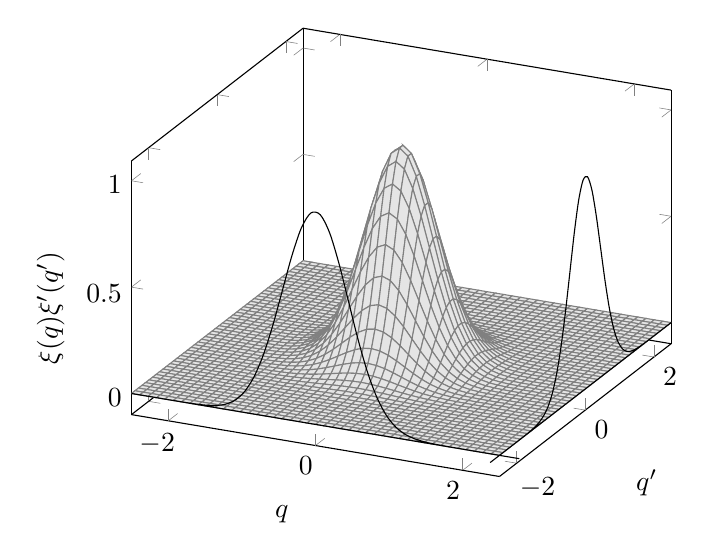
\begin{tikzpicture}[
    declare function = {f(\x,\y) = exp(-(\x^2+\y^2)/(4*0.1));}
]
\begin{axis}[
    xlabel = {$q$},
    ylabel = {$q'$},
    zlabel = {$\xi(q)\xi'(q')$}
]
    \addplot3[
        domain = -2.5:2.5,
        domain y = -2.5:2.5,
        samples = 45,
        samples y = 50,
        surf,
        fill = lightgray!40,
        faceted color = gray
    ]{f(\x, \y)};
    \addplot3[
        domain = -2.5:2.5,
        samples = 40,
        samples y = 40,
        smooth
    ](+2.5, \x, {f(\x, 0)});
    \addplot3[
        domain = -2.5:2.5,
        domain y = -2.5:2.5,
        samples = 40,
        samples y = 40,
        smooth
    ](\x, -2.5, {f(\x, 0)});
\end{axis}
\end{tikzpicture}

\end{document}